% Created by tikzDevice version 0.12 on 2019-02-12 15:48:00
% !TEX encoding = UTF-8 Unicode
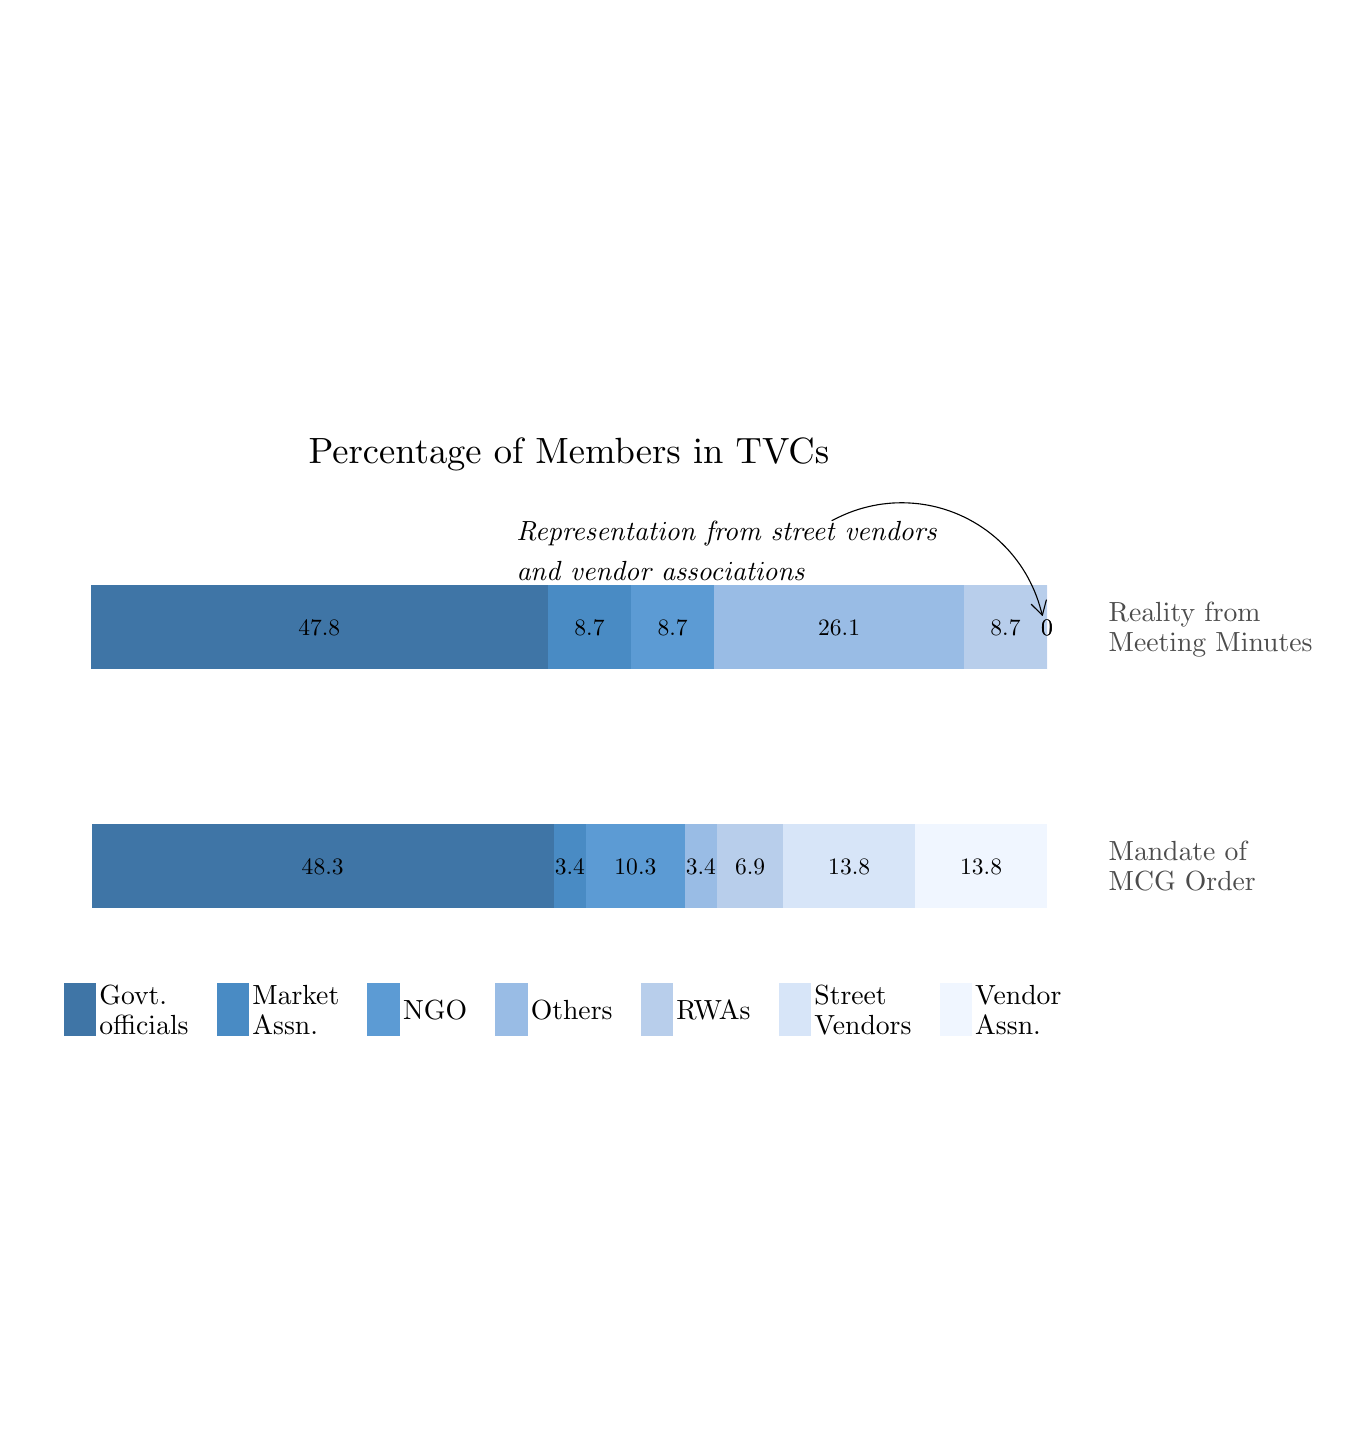
\begin{tikzpicture}[x=1pt,y=1pt]
\definecolor{fillColor}{RGB}{255,255,255}
\path[use as bounding box,fill=fillColor,fill opacity=0.00] (0,0) rectangle (469.75,505.89);
\begin{scope}
\path[clip] (  0.00,142.76) rectangle (469.75,363.13);
\definecolor{drawColor}{RGB}{255,255,255}
\definecolor{fillColor}{RGB}{255,255,255}

\path[draw=drawColor,line width= 0.6pt,line join=round,line cap=round,fill=fillColor] (  0.00,142.76) rectangle (469.76,363.13);
\end{scope}
\begin{scope}
\path[clip] (  5.50,151.01) rectangle (385.66,341.09);
\definecolor{fillColor}{RGB}{240,246,255}

\path[fill=fillColor] (320.68,187.73) rectangle (368.38,217.97);
\definecolor{fillColor}{RGB}{215,229,248}

\path[fill=fillColor] (272.99,187.73) rectangle (320.68,217.97);
\definecolor{fillColor}{RGB}{184,206,235}

\path[fill=fillColor] (249.15,187.73) rectangle (272.99,217.97);
\definecolor{fillColor}{RGB}{153,188,229}

\path[fill=fillColor] (237.40,187.73) rectangle (249.15,217.97);
\definecolor{fillColor}{RGB}{92,155,212}

\path[fill=fillColor] (201.80,187.73) rectangle (237.40,217.97);
\definecolor{fillColor}{RGB}{73,139,196}

\path[fill=fillColor] (190.05,187.73) rectangle (201.80,217.97);
\definecolor{fillColor}{RGB}{63,117,166}

\path[fill=fillColor] ( 23.13,187.73) rectangle (190.05,217.97);
\definecolor{fillColor}{RGB}{184,206,235}

\path[fill=fillColor] (338.31,274.13) rectangle (368.38,304.37);
\definecolor{fillColor}{RGB}{153,188,229}

\path[fill=fillColor] (248.11,274.13) rectangle (338.31,304.37);
\definecolor{fillColor}{RGB}{92,155,212}

\path[fill=fillColor] (218.04,274.13) rectangle (248.11,304.37);
\definecolor{fillColor}{RGB}{73,139,196}

\path[fill=fillColor] (187.98,274.13) rectangle (218.04,304.37);
\definecolor{fillColor}{RGB}{63,117,166}

\path[fill=fillColor] ( 22.78,274.13) rectangle (187.98,304.37);
\definecolor{fillColor}{RGB}{240,246,255}

\path[fill=fillColor] (368.38,274.13) rectangle (368.38,304.37);
\definecolor{fillColor}{RGB}{215,229,248}

\path[fill=fillColor] (368.38,274.13) rectangle (368.38,304.37);
\definecolor{drawColor}{RGB}{0,0,0}

\node[text=drawColor,anchor=base,inner sep=0pt, outer sep=0pt, scale=  0.85] at (344.53,199.91) {13.8};

\node[text=drawColor,anchor=base,inner sep=0pt, outer sep=0pt, scale=  0.85] at (296.84,199.91) {13.8};

\node[text=drawColor,anchor=base,inner sep=0pt, outer sep=0pt, scale=  0.85] at (261.07,199.91) {6.9};

\node[text=drawColor,anchor=base,inner sep=0pt, outer sep=0pt, scale=  0.85] at (243.27,199.91) {3.4};

\node[text=drawColor,anchor=base,inner sep=0pt, outer sep=0pt, scale=  0.85] at (219.60,199.91) {10.3};

\node[text=drawColor,anchor=base,inner sep=0pt, outer sep=0pt, scale=  0.85] at (195.92,199.91) {3.4};

\node[text=drawColor,anchor=base,inner sep=0pt, outer sep=0pt, scale=  0.85] at (106.59,199.91) {48.3};

\node[text=drawColor,anchor=base,inner sep=0pt, outer sep=0pt, scale=  0.85] at (353.34,286.31) {8.7};

\node[text=drawColor,anchor=base,inner sep=0pt, outer sep=0pt, scale=  0.85] at (293.21,286.31) {26.1};

\node[text=drawColor,anchor=base,inner sep=0pt, outer sep=0pt, scale=  0.85] at (233.08,286.31) {8.7};

\node[text=drawColor,anchor=base,inner sep=0pt, outer sep=0pt, scale=  0.85] at (203.01,286.31) {8.7};

\node[text=drawColor,anchor=base,inner sep=0pt, outer sep=0pt, scale=  0.85] at (105.38,286.31) {47.8};

\node[text=drawColor,anchor=base,inner sep=0pt, outer sep=0pt, scale=  0.85] at (368.38,286.31) {0};

\node[text=drawColor,anchor=base,inner sep=0pt, outer sep=0pt, scale=  0.85] at (368.38,286.31) {0};

\path[draw=drawColor,line width= 0.4pt,line join=round,line cap=round] (290.62,327.79) --
	(290.83,327.89) --
	(291.80,328.37) --
	(293.00,328.95) --
	(293.97,329.41) --
	(294.77,329.77) --
	(295.56,330.11) --
	(296.43,330.47) --
	(297.35,330.83) --
	(298.23,331.15) --
	(299.05,331.44) --
	(299.87,331.71) --
	(300.77,331.99) --
	(301.71,332.26) --
	(302.62,332.51) --
	(303.46,332.72) --
	(304.30,332.92) --
	(305.22,333.12) --
	(306.19,333.31) --
	(307.11,333.48) --
	(307.96,333.62) --
	(308.82,333.74) --
	(309.75,333.85) --
	(310.73,333.96) --
	(311.67,334.04) --
	(312.53,334.11) --
	(313.40,334.15) --
	(314.34,334.19) --
	(315.32,334.20) --
	(316.26,334.21) --
	(317.13,334.19) --
	(317.99,334.16) --
	(318.93,334.11) --
	(319.91,334.04) --
	(320.85,333.96) --
	(321.71,333.87) --
	(322.57,333.77) --
	(323.50,333.63) --
	(324.47,333.48) --
	(325.40,333.32) --
	(326.25,333.15) --
	(327.09,332.97) --
	(328.01,332.76) --
	(328.96,332.52) --
	(329.87,332.27) --
	(330.70,332.03) --
	(331.53,331.78) --
	(332.42,331.48) --
	(333.35,331.16) --
	(334.24,330.83) --
	(335.04,330.52) --
	(335.84,330.20) --
	(336.71,329.82) --
	(337.61,329.42) --
	(338.46,329.02) --
	(339.23,328.64) --
	(340.00,328.24) --
	(340.83,327.79) --
	(341.69,327.31) --
	(342.50,326.84) --
	(343.24,326.39) --
	(343.97,325.93) --
	(344.76,325.41) --
	(345.57,324.85) --
	(346.34,324.31) --
	(347.03,323.80) --
	(347.72,323.27) --
	(348.46,322.69) --
	(349.22,322.06) --
	(349.94,321.45) --
	(350.58,320.88) --
	(351.22,320.30) --
	(351.90,319.65) --
	(352.61,318.96) --
	(353.27,318.29) --
	(353.86,317.66) --
	(354.45,317.02) --
	(355.07,316.32) --
	(355.71,315.57) --
	(356.31,314.84) --
	(356.84,314.17) --
	(357.37,313.48) --
	(357.93,312.72) --
	(358.50,311.92) --
	(359.03,311.14) --
	(359.51,310.42) --
	(359.97,309.69) --
	(360.46,308.89) --
	(360.96,308.04) --
	(361.42,307.22) --
	(361.83,306.46) --
	(362.22,305.69) --
	(362.64,304.84) --
	(363.06,303.95) --
	(363.45,303.10) --
	(363.79,302.30) --
	(364.12,301.50) --
	(364.46,300.63) --
	(364.80,299.70) --
	(365.11,298.81) --
	(365.38,297.99) --
	(365.64,297.16) --
	(365.94,296.13) --
	(366.30,294.84) --
	(366.58,293.81) --
	(366.65,293.57);

\path[draw=drawColor,line width= 0.4pt,line join=round,line cap=round] (362.60,297.57) --
	(366.65,293.57) --
	(368.09,299.08);
\end{scope}
\begin{scope}
\path[clip] (  5.50,151.01) rectangle (385.66,341.09);
\definecolor{drawColor}{RGB}{0,0,0}

\node[text=drawColor,anchor=base west,inner sep=0pt, outer sep=0pt, scale=  1.00] at (176.57,320.59) {\itshape Representation from street vendors};

\node[text=drawColor,anchor=base west,inner sep=0pt, outer sep=0pt, scale=  1.00] at (176.57,306.19) {\itshape and vendor associations};
\end{scope}
\begin{scope}
\path[clip] (  0.00,  0.00) rectangle (469.75,505.89);
\definecolor{drawColor}{gray}{0.30}

\node[text=drawColor,anchor=base west,inner sep=0pt, outer sep=0pt, scale=  1.00] at (390.61,204.81) {Mandate of};

\node[text=drawColor,anchor=base west,inner sep=0pt, outer sep=0pt, scale=  1.00] at (390.61,194.01) {MCG Order};

\node[text=drawColor,anchor=base west,inner sep=0pt, outer sep=0pt, scale=  1.00] at (390.61,291.21) {Reality from};

\node[text=drawColor,anchor=base west,inner sep=0pt, outer sep=0pt, scale=  1.00] at (390.61,280.41) {Meeting Minutes};
\end{scope}
\begin{scope}
\path[clip] (  0.00,  0.00) rectangle (469.75,505.89);
\definecolor{fillColor}{RGB}{255,255,255}

\path[fill=fillColor] ( 12.83,141.20) rectangle (393.53,160.83);
\end{scope}
\begin{scope}
\path[clip] (  0.00,  0.00) rectangle (469.75,505.89);
\definecolor{drawColor}{RGB}{255,255,255}
\definecolor{fillColor}{gray}{0.95}

\path[draw=drawColor,line width= 5.7pt,line join=round,line cap=round,fill=fillColor] ( 12.83,141.20) rectangle ( 24.88,160.83);
\end{scope}
\begin{scope}
\path[clip] (  0.00,  0.00) rectangle (469.75,505.89);
\definecolor{fillColor}{RGB}{63,117,166}

\path[fill=fillColor] ( 13.02,141.39) rectangle ( 24.69,160.64);
\end{scope}
\begin{scope}
\path[clip] (  0.00,  0.00) rectangle (469.75,505.89);
\definecolor{drawColor}{RGB}{255,255,255}
\definecolor{fillColor}{gray}{0.95}

\path[draw=drawColor,line width= 5.7pt,line join=round,line cap=round,fill=fillColor] ( 68.15,141.20) rectangle ( 80.19,160.83);
\end{scope}
\begin{scope}
\path[clip] (  0.00,  0.00) rectangle (469.75,505.89);
\definecolor{fillColor}{RGB}{73,139,196}

\path[fill=fillColor] ( 68.34,141.39) rectangle ( 80.01,160.64);
\end{scope}
\begin{scope}
\path[clip] (  0.00,  0.00) rectangle (469.75,505.89);
\definecolor{drawColor}{RGB}{255,255,255}
\definecolor{fillColor}{gray}{0.95}

\path[draw=drawColor,line width= 5.7pt,line join=round,line cap=round,fill=fillColor] (122.60,141.20) rectangle (134.65,160.83);
\end{scope}
\begin{scope}
\path[clip] (  0.00,  0.00) rectangle (469.75,505.89);
\definecolor{fillColor}{RGB}{92,155,212}

\path[fill=fillColor] (122.79,141.39) rectangle (134.46,160.64);
\end{scope}
\begin{scope}
\path[clip] (  0.00,  0.00) rectangle (469.75,505.89);
\definecolor{drawColor}{RGB}{255,255,255}
\definecolor{fillColor}{gray}{0.95}

\path[draw=drawColor,line width= 5.7pt,line join=round,line cap=round,fill=fillColor] (168.77,141.20) rectangle (180.81,160.83);
\end{scope}
\begin{scope}
\path[clip] (  0.00,  0.00) rectangle (469.75,505.89);
\definecolor{fillColor}{RGB}{153,188,229}

\path[fill=fillColor] (168.95,141.39) rectangle (180.62,160.64);
\end{scope}
\begin{scope}
\path[clip] (  0.00,  0.00) rectangle (469.75,505.89);
\definecolor{drawColor}{RGB}{255,255,255}
\definecolor{fillColor}{gray}{0.95}

\path[draw=drawColor,line width= 5.7pt,line join=round,line cap=round,fill=fillColor] (221.33,141.20) rectangle (233.38,160.83);
\end{scope}
\begin{scope}
\path[clip] (  0.00,  0.00) rectangle (469.75,505.89);
\definecolor{fillColor}{RGB}{184,206,235}

\path[fill=fillColor] (221.52,141.39) rectangle (233.19,160.64);
\end{scope}
\begin{scope}
\path[clip] (  0.00,  0.00) rectangle (469.75,505.89);
\definecolor{drawColor}{RGB}{255,255,255}
\definecolor{fillColor}{gray}{0.95}

\path[draw=drawColor,line width= 5.7pt,line join=round,line cap=round,fill=fillColor] (271.23,141.20) rectangle (283.28,160.83);
\end{scope}
\begin{scope}
\path[clip] (  0.00,  0.00) rectangle (469.75,505.89);
\definecolor{fillColor}{RGB}{215,229,248}

\path[fill=fillColor] (271.42,141.39) rectangle (283.09,160.64);
\end{scope}
\begin{scope}
\path[clip] (  0.00,  0.00) rectangle (469.75,505.89);
\definecolor{drawColor}{RGB}{255,255,255}
\definecolor{fillColor}{gray}{0.95}

\path[draw=drawColor,line width= 5.7pt,line join=round,line cap=round,fill=fillColor] (329.35,141.20) rectangle (341.40,160.83);
\end{scope}
\begin{scope}
\path[clip] (  0.00,  0.00) rectangle (469.75,505.89);
\definecolor{fillColor}{RGB}{240,246,255}

\path[fill=fillColor] (329.54,141.39) rectangle (341.21,160.64);
\end{scope}
\begin{scope}
\path[clip] (  0.00,  0.00) rectangle (469.75,505.89);
\definecolor{drawColor}{RGB}{0,0,0}

\node[text=drawColor,anchor=base west,inner sep=0pt, outer sep=0pt, scale=  1.00] at ( 25.88,152.97) {Govt.};

\node[text=drawColor,anchor=base west,inner sep=0pt, outer sep=0pt, scale=  1.00] at ( 25.88,142.17) {officials};
\end{scope}
\begin{scope}
\path[clip] (  0.00,  0.00) rectangle (469.75,505.89);
\definecolor{drawColor}{RGB}{0,0,0}

\node[text=drawColor,anchor=base west,inner sep=0pt, outer sep=0pt, scale=  1.00] at ( 81.19,152.97) {Market};

\node[text=drawColor,anchor=base west,inner sep=0pt, outer sep=0pt, scale=  1.00] at ( 81.19,142.17) {Assn.};
\end{scope}
\begin{scope}
\path[clip] (  0.00,  0.00) rectangle (469.75,505.89);
\definecolor{drawColor}{RGB}{0,0,0}

\node[text=drawColor,anchor=base west,inner sep=0pt, outer sep=0pt, scale=  1.00] at (135.65,147.57) {NGO};
\end{scope}
\begin{scope}
\path[clip] (  0.00,  0.00) rectangle (469.75,505.89);
\definecolor{drawColor}{RGB}{0,0,0}

\node[text=drawColor,anchor=base west,inner sep=0pt, outer sep=0pt, scale=  1.00] at (181.81,147.57) {Others};
\end{scope}
\begin{scope}
\path[clip] (  0.00,  0.00) rectangle (469.75,505.89);
\definecolor{drawColor}{RGB}{0,0,0}

\node[text=drawColor,anchor=base west,inner sep=0pt, outer sep=0pt, scale=  1.00] at (234.38,147.57) {RWAs};
\end{scope}
\begin{scope}
\path[clip] (  0.00,  0.00) rectangle (469.75,505.89);
\definecolor{drawColor}{RGB}{0,0,0}

\node[text=drawColor,anchor=base west,inner sep=0pt, outer sep=0pt, scale=  1.00] at (284.28,152.97) {Street};

\node[text=drawColor,anchor=base west,inner sep=0pt, outer sep=0pt, scale=  1.00] at (284.28,142.17) {Vendors};
\end{scope}
\begin{scope}
\path[clip] (  0.00,  0.00) rectangle (469.75,505.89);
\definecolor{drawColor}{RGB}{0,0,0}

\node[text=drawColor,anchor=base west,inner sep=0pt, outer sep=0pt, scale=  1.00] at (342.40,152.97) {Vendor};

\node[text=drawColor,anchor=base west,inner sep=0pt, outer sep=0pt, scale=  1.00] at (342.40,142.17) {Assn.};
\end{scope}
\begin{scope}
\path[clip] (  0.00,  0.00) rectangle (469.75,505.89);
\definecolor{drawColor}{RGB}{0,0,0}

\node[text=drawColor,anchor=base,inner sep=0pt, outer sep=0pt, scale=  1.32] at (195.58,348.54) {Percentage of Members in TVCs};
\end{scope}
\end{tikzpicture}
